\begin{center}\begin{LARGE} \end{LARGE}\end{center}

\newpage
\begin{problem}{i}
Write the gradient and Heissan matrix of the following formula.
\textcolor{red}{[10pts]}$$\mathbf{x}^{\mathrm{T}}\mathbf{Ax}+\mathbf{b}^{\mathrm{T}}\mathbf{x}+\mathrm{c}\quad(\mathbf{A}\in\mathbf{R^{n*n}}, \mathbf{b}\in\mathbf{R^{n}}, \mathrm{c}\in\mathbf{R})$$
\end{problem}

    %type your answer here
    Let $f(\mathbf{x})=\mathbf{x}^{\mathrm{T}}\mathbf{Ax}+\mathbf{b}^{\mathrm{T}}\mathbf{x}+\mathrm{c}$\\
   
    1. the gradient of the formula is\\
    $\nabla f=\dfrac{\partial f}{\partial\mathbf{x}}=(\mathbf{A+A}^T)\mathbf{x}+\mathbf{b}$\\

    2. the Heissan matrix of the formula is\\
    $\nabla^2 f=\nabla(\nabla f)=\dfrac{\partial(\nabla f)}{\partial\mathbf{x}^T}=\mathbf{A}+\mathbf{A}^T$\\

\newpage
\begin{problem}{ii}
Write the gradient and Heissan matrix of the following formula.
\textcolor{red}{[10pts]}$$\left\|\mathbf{Ax}-\mathbf{b}\right\|^{2}_{2}\quad(\mathbf{A}\in\mathbf{R^{m*n}}, \mathbf{b}\in\mathbf{R^{m}})$$
\end{problem}

    %type your answer here
    Let $f(\mathbf{x})=\left\|\mathbf{Ax}-\mathbf{b}\right\|^{2}_{2}=(\mathbf{Ax}-\mathbf{b})^T(\mathbf{Ax}-\mathbf{b})=\mathbf{x^TA^TAx}-\mathbf{2x^TA^Tb}+\mathbf{b^Tb}$\\
    1. the gradient of the formula is\\
    $\nabla f=\dfrac{\partial f}{\partial\mathbf{x}}=\mathbf{2A^TAx}-\mathbf{2A^Tb}$\\

    2. the Heissan matrix of the formula is\\
    $\nabla^2 f=\nabla(\nabla f)=\dfrac{\partial(\nabla f)}{\partial\mathbf{x}^T}=\mathbf{2A^TA}$\\

\newpage    
\begin{problem}{iii}
Convert the following problem to linear programming.
\textcolor{red}{[10pts]}$$\min_{\mathbf{x}\in\mathbf{R^{n}}}\left\|\mathbf{Ax}-\mathbf{b}\right\|_{1}+\left\|\mathbf{x}\right\|_{\infty}\quad(\mathbf{A}\in\mathbf{R^{m*n}}, \mathbf{b}\in\mathbf{R^{m}})$$
\end{problem}

    %type your answer here
    1. for the first part,\\
    let $z_i = |\mathbf{r_i}^T\mathbf{x}-b_i|$, where $\mathbf{r_i}\textcolor{red}{^T}$ is the $i$-th row of the matrix $\mathbf{A}$, and $b_i$ is the $i$-th element in the column vector $\mathbf{b}$.\\
    So $\left\|\mathbf{Ax}-\mathbf{b}\right\|_1=\sum\limits_{i=1}^m z_i$\\
    And $-z_i \leq \mathbf{r_i}^T\mathbf{x}-b_i \leq z_i$ and $z_i \geq 0$\\

    2. for the second part,\\
    let $w = \max\limits_{i=1,2,\cdots,n}|x_i|$, where $x_i$ is the $i$-th element in the vector $\mathbf{x}$\\
    So $\left\|\mathbf{x}\right\|_\infty=w$\\
    And $-w \leq x_i \leq w$\\
    
    So combine the two parts, we convert the problem into the linear programming:\\
    \begin{equation*}
        \begin{aligned}
            \min_{\mathbf{x}\in\mathbf{R^{n}}}\quad & (\sum\limits_{i=1}^m z_i) + w\\
            subject\ to \quad & -z_i \leq \mathbf{r_i}^T\mathbf{x}-b_i \leq z_i, \quad i=1,2,\cdots,m\\
            & -w \leq x_i\leq w, \quad i=1,2,\cdots,n\\
            & z_i \geq 0, \quad i=1,2,\cdots,m\\
            & w\geq 0\\
        \end{aligned}
    \end{equation*}


\newpage
\begin{problem}{vi}
Proof the convergence rates of the following point sequences.
\textcolor{red}{[30pts]}$$\mathbf{x^{\mathrm{k}}}=\frac{\mathrm{1}}{\mathrm{k}}$$$$\mathbf{x^{\mathrm{k}}}=\frac{\mathrm{1}}{\mathrm{k!}}$$$$\mathbf{x^{\mathrm{k}}}=\frac{\mathrm{1}}{\mathrm{2^{2^{k}}}}$$(Hint: Given two iterates $\mathbf{x^{\mathrm{k+1}}}$ and $\mathbf{x^{\mathrm{k}}}$, and its limit point $\mathbf{x^{\mathrm{*}}}$, there exists real number $\mathrm{q > 0}$, satisfies $$\lim_{\mathrm{k\rightarrow\infty}}\frac{\left\|\mathbf{x^{\mathrm{k+1}}}-\mathbf{x^{\mathrm{*}}}\right\|}{\left\|\mathbf{x^{\mathrm{k}}}-\mathbf{x^{\mathrm{*}}}\right\|} = \mathrm{q}$$ if $\mathrm{0<q<1}$, then the point sequence Q-linear convergence; if $\mathrm{q=1}$, then the point sequence Q-sublinear convergence; if $\mathrm{q=0}$, then the point sequence Q-superlinear convergence)
\end{problem}

    %type your answer here
    1. for $\mathbf{x}^k = \dfrac{1}{k}$:\\
    since $\lim\limits_{k\to\infty}\mathbf{x}^k = 0$, so $\mathbf{x}^*=0$\\
    so $\lim\limits_{k\to\infty}\dfrac{\left\|\mathbf{x}^{k+1}-\mathbf{x}^*\right\|}{\left\|\mathbf{x}^k-\mathbf{x}^*\right\|}=\lim\limits_{k\to\infty}\dfrac{\left\|\dfrac{1}{k+1}\right\|}{\left\|\dfrac{1}{k}\right\|}=\lim\limits_{k\to\infty}\dfrac{k}{k+1}=1$\\
    i.e. $q=1$.
    so the point sequence is Q-sublinear convergence.\\

    2. for $\mathbf{x}^k = \dfrac{1}{k!}$:\\
    since $\lim\limits_{k\to\infty}\mathbf{x}^k = 0$, so $\mathbf{x}^*=0$\\
    so $\lim\limits_{k\to\infty}\dfrac{\left\|\mathbf{x}^{k+1}-\mathbf{x}^*\right\|}{\left\|\mathbf{x}^k-\mathbf{x}^*\right\|}=\lim\limits_{k\to\infty}\dfrac{\left\|\dfrac{1}{(k+1)!}\right\|}{\left\|\dfrac{1}{k!}\right\|}=\lim\limits_{k\to\infty}\dfrac{k!}{(k+1)!}=\lim\limits_{k\to\infty}\dfrac{1}{k+1}=0$\\
    i.e. $q=0$. 
    so the point sequence is Q-superlinear convergence.\\

    3. for $\mathbf{x}^k = \dfrac{1}{2^{2^k}}$:\\
    since $\lim\limits_{k\to\infty}\mathbf{x}^k = 0$, so $\mathbf{x}^*=0$\\
    so $\lim\limits_{k\to\infty}\dfrac{\left\|\mathbf{x}^{k+1}-\mathbf{x}^*\right\|}{\left\|\mathbf{x}^k-\mathbf{x}^*\right\|}=\lim\limits_{k\to\infty}\dfrac{\left\|\dfrac{1}{2^{2^{k+1}}}\right\|}{\left\|\dfrac{1}{2^{2^k}}\right\|}=\lim\limits_{k\to\infty}\dfrac{2^{2^k}}{2^{2^{k+1}}}=\lim\limits_{k\to\infty}{2^{-2^k}}=0$\\
    i.e. $q=0$.
    so the point sequence is Q-superlinear convergence.\\

    So above all, the point sequence $\mathbf{x}^k = \dfrac{1}{k}$ is Q-sublinear convergence, the point sequence $\mathbf{x}^k = \dfrac{1}{k!}$ and $\mathbf{x}^k = \dfrac{1}{2^{2^k}}$ are Q-superlinear convergence.\\


\newpage
\begin{problem}{v}
Select the Haverly Pool Problem or the Horse Racing Problem in the courseware, compile the program using AMPL model language and submit it to \url{https://neos-server.org/neos/solvers/index.html}.(Hint: both AMPL solver and NEOS solver can be used, please indicate the type of solver used in the submitted job, show the solution results (eg: screenshots attached to the PDF file), and submit the source code together with the submitted job, please package as .zip file, including your PDF and source code.)
\textcolor{red}{[40pts]}
\end{problem}
    
    Select the Haverly Pooling Problem.\\
    The codes are in the additional files.\\
    And since the problem is a bilinear problem, i.e. a non linear problem,
    so I used the the LOQO solver in the nonlinearly constrianed optimization to solve the problem.\\
    The results are as follows:\\

    \begin{figure}[htbp]
        \centering
        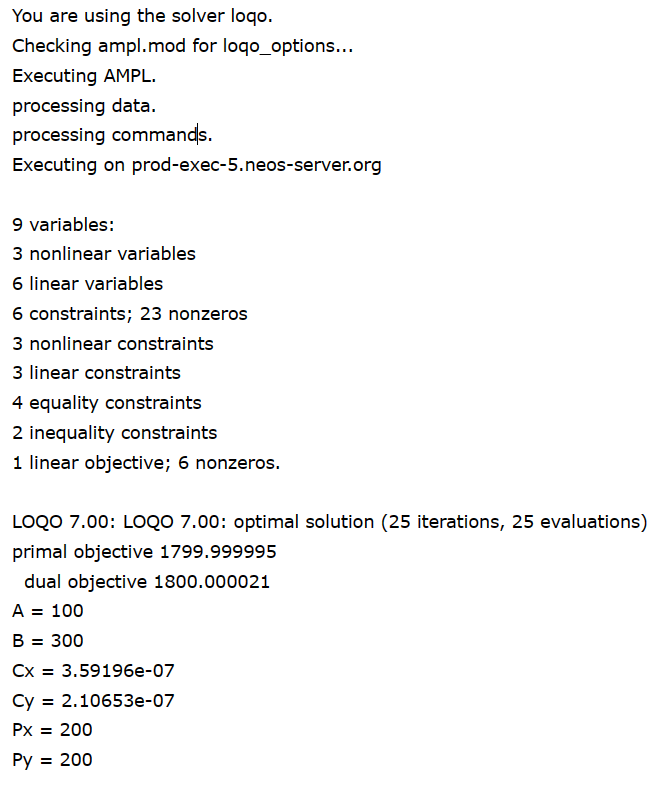
\includegraphics[width=0.7\textwidth]{../result/result.png} % 
        \caption{The results of the Haverly Pooling Problem}
    \end{figure}